\documentclass[./bab_3.tex]{subfiles}
\begin{document}
  \section{Pemodelan yang digunakan}
  \subsection{Topologi Jaringan}
  \paragraph*{}Pemodelan yang digunakan merepresentasikan
  susunan dari komputer yang ada pada jaringan. Pada
  perancangan jaringan yang akan diimplementasikan mitmproxy
  menggunakan pemodelan topologi jaringan.

  \begin{figure}[hbt!]
  \centering
    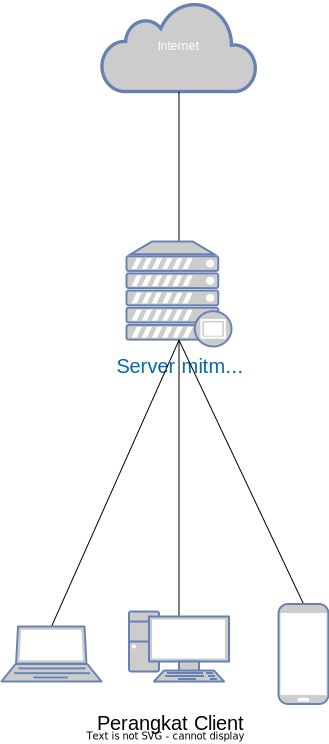
\includegraphics[scale=0.4]{topology01.png}
    \caption{Topologi Jaringan Sistem}
  \end{figure}

  \paragraph*{}Sistem yang dibuat merupakan server proxy, sehingga
  perangkat-perangkat client akan terhubung ke proxy
  terlebih dahulu sebelum terhubung pada internet.

  \subsection{Algoritma}
  \begin{figure}[hbt!]
  \centering
    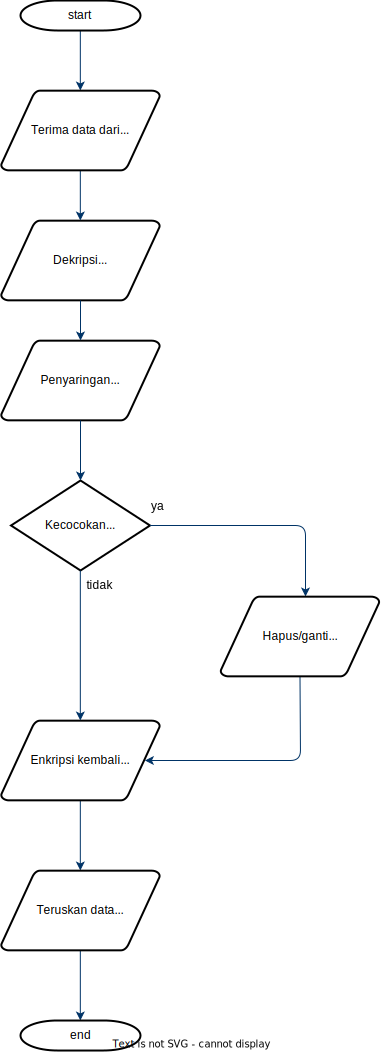
\includegraphics[scale=0.4]{flowchart01.png}
    \caption{Algoritma Sistem Mitmproxy}
  \end{figure}

  \paragraph*{}Untuk melakukan enkripsi diperlukan
  \textit{certificate}. \textit{Certificate} dapat diperoleh
  dari yang sudah dibuat oleh mitmproxy, atau dapat juga
  dibuat dengan menggunakan OpenSSL. Untuk membuat
  \textit{certificate} dengan menggunakan OpenSSL, Gunakan
  perintah:

  \mintinline[fontsize=\footnotesize]{bash}{openssl req -key private_key -x509 -new -days days -out namafile}

  Setelah \textit{certificate} didapatkan,
  \textit{certificate} tersebut perlu untuk diinstall di
  perangkat \textit{client}.

  \paragraph*{}Sedangkan untuk melakukan penyaringan konten,
  memanfaatkan \textit{library} Python BeautifulSoup dan
  library JSON \textit{built-in} di Python. \textit{Library}
  BeautifulSoup digunakan untuk mencari komponen-komponen
  HTML secara idiomatis, yang digunakan untuk menampilkan
  halaman web.
  Sedangkan library JSON digunakan untuk
  mem-\textit{parsing} data JSON, karena ada beberapa
  halaman web yang memanfaatkan FetchAPI untuk mengunduh
  kontennya. FetchAPI biasanya berkomunikasi dengan format
  data JSON. Dengan menggunakan \textit{library} ini
  diharapkan pembuatan script python untuk memfilter konten
  yang ditentukan menjadi mudah, karena tidak harus mencari
  komponen-komponen HTML dengan menuliskan
  \textit{regular-expression}.

  \paragraph*{} Berikut ini merupakan contoh penggunaan \textit{library} BeautifulSoup.

  \begin{minted}[frame=lines, framesep=2mm, baselinestretch=1.2, bgcolor=LightGray, fontsize=\footnotesize, linenos]{python}
from mitmproxy import http
from mitmproxy import ctx
from bs4 import BeautifulSoup

class ReplaceHTML:
  filter = "ads"

  def response(self, flow: http.HTTPFlow):
    html = BeautifulSoup(flow.response.content, "lxml")
    for div in html.find_all('div', attrs={"class":filter}):
      div.decompose()
    flow.response.content = str(html).encode("utf8")

addons = [ReplaceHTML()]
  \end{minted}

  \paragraph*{} Kode di atas menggunakan library yang
  disediakan oleh mitmproxy, dan BeautifulSoup. Di kode
  tersebut terdapat \textit{events} response.
  \textit{Events} ini dipicu sebelum response sampai di
  perangkat \textit{client}. Kemudian \textit{content} dari
  response di-\textit{parsing} oleh BeautifulSoup menggunakan
  lxml. Setelah itu dilakukan perulangan yang akan mencari
  elemen 'div' yang mengandung kata \textit{"ads"} di
  kelasnya, dan menghapus elemen tersebut. Setelah itu
  content yang sudah diolah tadi, dikembalikan menjadi
  bentuk teks, dan diteruskan ke perangkat client.

  \begin{minted}[frame=lines, framesep=2mm, baselinestretch=1.2, bgcolor=LightGray, fontsize=\footnotesize, linenos]{python}
from mitmproxy import ctx
from mitmproxy import http
import json

class ReplaceJSON
  def response(flow: http.HTTPFlow) -> None:
      if flow.request.url.startswith("http://example.com/"):
          data = json.loads(flow.response.get_text())
          data["ads"][0]["advertisement"] = False
          flow.response.text = json.dumps(data)

addons = [ReplaceJSON()]
  \end{minted}

  \paragraph*{} Kode di atas merupakan contoh penggunaan
  \textit{library} JSON, sama seperti kode sebelumnya, kode
  ini menggunakan \textit{response}. Dalam kode ini jika url
  yang diakses merupakan "example.com" maka data akan
  di-\textit{parsing} dengan menggunakan library json.
  Kemudian data JSON yang dari \textit{advertisement} akan
  diubah menjadi \textit{False}.

\end{document}
